\section{RQ3: Engagement with Misinformation and Authentic News}
Having explored how misinformation on Reddit promotes toxic, insular, and polarized environments on Reddit, we finally turn to understand these factors' role in user engagement with misinformation and authentic news.  Namely having seen that misinformation produces more toxic and politically uncivil environments, do these environments lead to more engagement with misinformation? Various works have found that toxic and polarized environments often provoke engagement from users as they get ``outraged'' by the presented content~\cite{kim2021distorting,gallacher2021online}. In this final section, we seek to determine how different communities and different community norms affect the rates at which misinformation and authentic news get interactions on Reddit.

\subsection{Experimental Setup} To understand user interactions and engagement with misinformation and authentic news URL submissions, we utilize the number of comments that each submission receives. We utilize the number of comments rather than the number of upvotes/downvotes, due to the unreliability of Pushshift's data for this particular submission characteristic. While Pushshift often can acquire most submissions and comments, it often fails to keep up-to-date information about the number of votes a given submission receives~\cite{baumgartner2020pushshift}. This is largely due to the high rate at which submission upvotes/downvotes change. We thus use the more stable and reliable ``number of comments'' number to determine user engagement with a given submission. We lastly note that to properly model the number of comments, we remove comments from Reddit ``auto moderator'' accounts (often subreddits have auto moderators that automatically comment on submissions). We thus consider the number of comments from ``real world'' users. 

\begin{figure}
\begin{minipage}[l]{0.4\textwidth}
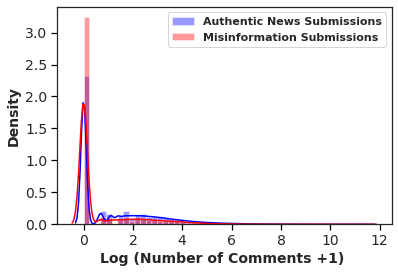
\includegraphics[width=1\columnwidth]{figures/num_submissions.png} 
\end{minipage}
\begin{minipage}[l]{0.35\textwidth}
\caption{\textbf{Log of number of submissions for misinformation and authentic news submissions}--- A large majority of submissions do not receive  comments.\label{fig:num_comments}}
\end{minipage}

\end{figure}


To model the count data of the number of comments on given submissions, we utilize a zero-inflated negative binomial regression~\cite{ridout2001score}. Within our regression, each observation represents a single submission and the number of comments it garnered. We specifically utilize a zero-inflated negative binomial regression as it appropriately models our set of count data. Unlike a Poisson model, which is often utilized to model count data, negative binomial regressions do not make the strong assumption that the mean of the data is equal to the variance~\cite{morina2022web}. Given that some submissions garner thousands of comments while others garner none, utilizing a Poisson model would be somewhat inappropriate. We further utilize the zero-inflated version of this regression given the heavy preponderance of submissions that do not receive any comments. After removing comments from auto moderators, as depicted in Figure~\ref{fig:num_comments}, 54.5\% of submissions within our dataset did not receive any comments. A normal negative binomial model would thus be unable the correctly model this behavior. 

\begin{table}[b]
\centering
\begin{tabular}{lll}
\toprule
   \multicolumn{3}{c}{\large Number of Comments on Misinfo Submissions}          \\
   \toprule
                                  & {Zero Inflated}  & {Negative Binomial }  \\
                      &       \footnotesize{negative coefficient = } &  \footnotesize{positive coefficient = }\\
                      &       \footnotesize{more likely to get comments} &  \footnotesize{more comments}\\
      \midrule
      Intercept              & 5.3146*** & 3.290***  \\               
      \midrule
      Absolute User Polarization               & -7.2400***  & -4.5838***  \\
      \midrule
      Absolute Subreddit Polarization              & 5.3818 &0.9658** \\
    \midrule
       Subreddit Toxicity & -2.5780***   & 5.3042*** \\
      \midrule
       User Toxicity &   -11.3991  *** &  -11.8022***\\
      \midrule
      Average Subreddit Comments &  -7.0379 *** & 1.0354***  \\
\bottomrule
& $^\ast p<0.05; \;  ^{**} p<0.01; \; ^{***}p<0.001$ \\
\end{tabular}
\caption{Fit of our zero-inflated negative binomial regression on the number of comments on our set of misinformation URL submissions across different subreddits.} 
\label{tbl:misinfo-fit}
\end{table}
\begin{table}[b]
\centering
\begin{tabular}{lll}
\toprule
   \multicolumn{3}{c}{\large Number of Comments on Authentic News Submissions}          \\
   \toprule
                            & {Zero Inflated}  & {Negative Binomial }  \\
                      &       \footnotesize{negative coefficient = } &  \footnotesize{positive coefficient = }\\
                      &       \footnotesize{more likely to get comments} &  \footnotesize{more comments}\\
      \midrule
      Intercept              & 3.7182***  &2.7577*** \\               
      \midrule
     Absolute User Polarization               & -2.7390***  & -3.0487 ***  \\
      \midrule
      Absolute Subreddit Polarization              & 5.9227*** &1.4898 *** \\
    \midrule
      Subreddit Toxicity & 6.1866***  & 13.1317*** \\
      \midrule
       User Toxicity &   -14.8969*** &  --8.0695***\\
      \midrule
      Average Subreddit Comments &  -6.4304*** & 0.6121***  \\
\bottomrule
& $^\ast p<0.05; \;  ^{**} p<0.01; \; ^{***}p<0.001$ \\
\end{tabular}
\caption{Fit of our zero-inflated negative binomial regression on the number of comments on our set of authentic news URL submissions across different subreddits.} 
\label{tbl:mainstream-fit}
\end{table}
Zero-inflated negative binomial regressions return two sets of coefficients. One set of coefficients, the zero-inflated coefficients, estimated using logistic regression, give the probability that the given submission would receive 0 comments as a function of the covariates. Positive coefficients for these zero-inflated coefficients indicate that increases in the predictor variable make a receiving 0 comment more likely. Thus the more negative a coefficient, the more the given covariate correlates with inducing at least 1 comment. The second set of coefficients, the negative binomial coefficients, model the number of comments as a function of the covariates. For these coefficients, positive coefficients indicate that the larger the corresponding covariate, the more comments that submission was likely to have received.  We thus, in our analysis, can understand how different covariates affect the probability that a given submission will receive \textit{any} comments \emph{and} how these same covariates affect the number of comments received. 

For data, we model the number of garnered comments for both our set of 47,822 misinformation submissions and 787,603 authentic news submissions. As factors influencing the number of comments, we utilize (1) the submitter's polarization, (2) the subreddit's polarization, (3) the toxicity norm of the subreddit, (4) the submitter's toxicity norm, and (5) the average number of comments with the subreddit the submission was posted in. 


\subsection{Results}  Before engaging in a thorough analysis of the fits of our zero-inflated negative binomials, we first perform a spot-check on the results. We ensure that the higher the average amount of comments in a given subreddit the more likely a submission is to get comments and that this average correlates with more comments on given submissions. In other words, we check that submissions in subreddits where users comment more, also received more comments. As seen in both Tables~\ref{tbl:misinfo-fit} and~\ref{tbl:mainstream-fit}, for both misinformation and authentic news Reddit submissions as the average number of comments in a particular subreddit increases, (1) the more likely a submission is to get comments at all and (2) the more comments it is likely to get. Having observed this behavior, we now move to examine the rest of the covariates within our fits. 

\paragraph{User Polarization} We observe similar behavior for the effect of the posting user political polarization on the number of comments that the submissions received. For both authentic news and misinformation submissions, we see that as the submission's submitter becomes more politically polarized (\textit{i.e.} moves to the political extremes on the political left or right), the more likely their posts are to receive comments. With zero-inflated coefficients of -7.24 for misinformation submissions and -2.74 for authentic news submissions, we see that this is particularly true for misinformation submissions. This largely agrees with prior work that has shown that highly polarized users are likely to provoke and garner comments on social media platforms~\cite{kim2021distorting,howard2019ira}

However, despite highly polarized users being able to attract at least one comment, we further observe that for both authentic news and misinformation submissions as the posting user becomes more politically polarized, the fewer comments their post is likely to receive. This appears to indicate that in the case of misinformation and authentic news submission, Reddit users are perhaps being ``turned off'' and engaging less with highly polarized users~\cite{hetherington2008turned}compared to more politically neutral users.

\paragraph{Subreddit Polarization} While we are unable to conclude using our model whether subreddit polarization has an effect on misinformation submissions, we find that for authentic news submissions the more politically polarized a subreddit is, the less likely anyone is to comment on authentic news submissions. This may indicate as a whole that authentic news submissions do not ordinarily get much traction on highly polarized subreddits. Rather, as documented by Wang \textit{et al.}~\cite{wang2021multi} subreddits like these often ignore more trustworthy sources. We thus find that the insular nature of more partisan subreddits may be inducing them to largely ignore authentic news submissions when they appear within their subreddit.
 
In contrast, for both misinformation and authentic news submissions, we find that as polarization goes up, the more comments given submissions are likely to garner. This reflects that \emph{when} authentic news and misinformation submissions are noticed, the more polarized the environment, the more users seem to comment and engage with submissions~\cite{kim2021distorting}.
 
\paragraph{Subreddit Toxicity}
Looking at the subreddit toxicity, we see a marked difference between authentic news submissions and misinformation submissions. We see, notably, for misinformation submissions, the more toxic a subreddit is, the more likely the submission is to get comments. In contrast, for authentic news submissions, the more toxic the subreddit, the more likely the submission is to not get any comments at all. This appears to reflect that authentic news submissions may often not have ``clickbait'' titles that induce readers to often angrily engage with  material~\cite{chen2015misleading,potthast2016clickbait}. In contrast, oftentimes misinformation websites often post inflammatory articles designed to engender angst in their readership. For example, with regards to the COVID-19 pandemic, the misinformation website infowars.com~\cite{starbird2018ecosystem}  recently published a report entitled \textit{``Wake Up! Even The Masks Made You Sick''!} As subreddits get more toxic, we thus see that their users are more likely to engage with articles such as this. 
 
Similar to polarization, for both misinformation and authentic news submissions, we find that as subreddit toxicity goes up, the more comments given submissions are likely to garner. This again reflects that \emph{when} authentic news and misinformation submissions are noticed, the more toxic the environment the more users seem to comment and engage with submissions. We thus see that though authentic news submissions are more often ignored in toxic subreddits when compared to misinformation, when they are noticed, toxic environments produce more engagement with both types of submission. 

\paragraph{User Toxicity}  Finally, looking at user toxicity, we see similar behaviors for both authentic news and misinformation submissions. Most notably, as users become more toxic for both misinformation and authentic news submission, the more likely they are to provoke at least one comment. We thus see that user toxicity is a means by which to gain engagement from posting news articles generally. However, again in both cases, we see that while user toxicity often provokes at least one person to react, we see that this toxicity, often does not lead to more comments on the whole. As found in prior work, toxic users, while often sparking retorts as other users become enraged, also create unhealthy, short, and otherwise bad conversational outcomes~\cite{saveski2021structure,kumar2021designing}. This result largely matches our definition of individual toxicity as comments that \textit{are likely to make one leave the discussion} from Section~\ref{sec:misinformation-defintion}. We thus as a whole see that as entire communities/subreddit becomes more toxic, they are more likely to engage with materials more thoroughly, but as individual users become more toxic, they are more likely to end and otherwise shorten conversations. 






